
\documentclass[tikz, border=10pt]{standalone}
\usepackage{tikz}
\usepackage{graphicx}
\usetikzlibrary{positioning, shadows, calc, shapes}

\begin{document}
\section{U-FNO Architecture}
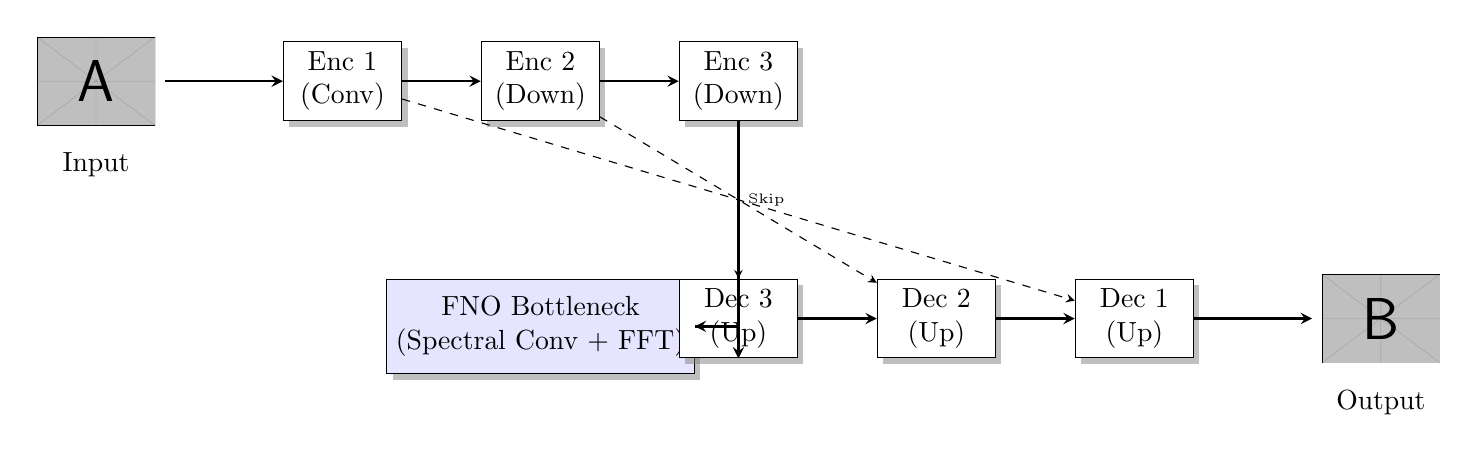
\begin{tikzpicture}[
    node distance=1.2cm,
    block/.style={draw, rectangle, minimum height=1.0cm, minimum width=1.5cm, align=center, fill=white, drop shadow},
    fno/.style={draw, rectangle, minimum height=1.2cm, minimum width=3.0cm, align=center, fill=blue!10, drop shadow},
    arrow/.style={->, >=stealth, thick},
    skip/.style={->, >=stealth, dashed}
]
    % Encoder
    \node (input) {\includegraphics[width=1.5cm]{example-image-a}};
    \node[below=0.1cm of input] {Input};

    \node[block, right=1.5cm of input] (enc1) {Enc 1\\(Conv)};
    \node[block, right=1.0cm of enc1] (enc2) {Enc 2\\(Down)};
    \node[block, right=1.0cm of enc2] (enc3) {Enc 3\\(Down)};

    % Bottleneck (FNO)
    \node[fno, below=2.0cm of enc2] (bottleneck) {FNO Bottleneck\\(Spectral Conv + FFT)};

    % Decoder
    \node[block, below=2.0cm of enc3] (dec3) {Dec 3\\(Up)};
    \node[block, right=1.0cm of dec3] (dec2) {Dec 2\\(Up)};
    \node[block, right=1.0cm of dec2] (dec1) {Dec 1\\(Up)};
    
    \node[right=1.5cm of dec1] (output) {\includegraphics[width=1.5cm]{example-image-b}};
    \node[below=0.1cm of output] {Output};

    % Encoder Flow
    \draw[arrow] (input) -- (enc1);
    \draw[arrow] (enc1) -- (enc2);
    \draw[arrow] (enc2) -- (enc3);
    
    % To Bottleneck
    \draw[arrow] (enc3) |- (bottleneck);
    
    % To Decoder
    \draw[arrow] (bottleneck) -| (dec3);
    
    % Decoder Flow
    \draw[arrow] (dec3) -- (dec2);
    \draw[arrow] (dec2) -- (dec1);
    \draw[arrow] (dec1) -- (output);

    % Skip Connections (U-Net style)
    % Ideally horizontal if layout permits, here we use simple curves or straight lines
    % We adjust positions to make them look like U-Net if we used a standard U-layout, 
    % but here we used a wrapped layout. Let's try to align Decoders under Encoders for better skips.
    
    % Re-positioning for U-shape alignment
    % Let's use coordinate extraction to align Dec under Enc
    % But we already placed them. Let's rely on relative placement above.
    % Actually, let's force alignment:
    % enc1 -- enc2 -- enc3
    % dec1 -- dec2 -- dec3
    % Skip: enc3 -> dec3 (if matched), enc2 -> dec2...
    
    % Let's redraw lines for skips
    % Note: In this specific layout (Enc top row, Dec bottom row), skips are vertical
    \draw[skip] (enc3) -- node[right, font=\tiny] {Skip} (dec3);
    \draw[skip] (enc2) -- (dec2);
    \draw[skip] (enc1) -- (dec1);

\end{tikzpicture}
\end{document}
